\documentclass[border=2mm]{standalone}
\usepackage{pgfplots, pgfplotstable}
\usepackage{amsmath,nicefrac}

\makeatletter
	\long\def\ifnodedefined#1#2#3{%
	    \@ifundefined{pgf@sh@ns@#1}{#3}{#2}%
	}

	\pgfplotsset{
	    discontinuous/.style={
	    scatter,
	    scatter/@pre marker code/.code={
		\ifnodedefined{marker}{
			\pgfpointdiff{\pgfpointanchor{marker}{center}}%
			 {\pgfpoint{0}{0}}%
			 \ifdim\pgf@y>0pt
			    \tikzset{options/.style={mark=*, fill=white}}
			    \draw [densely dashed] (marker-|0,0) -- (0,0);
			    \draw plot [mark=*] coordinates {(marker-|0,0)};
			 \else
			    \tikzset{options/.style={mark=none}}
			 \fi
		}{
			\tikzset{options/.style={mark=none}}        
		}
		\coordinate (marker) at (0,0);
		\begin{scope}[options]
	    },
	    scatter/@post marker code/.code={\end{scope}}
	    }
	}
\makeatother

\begin{document}
	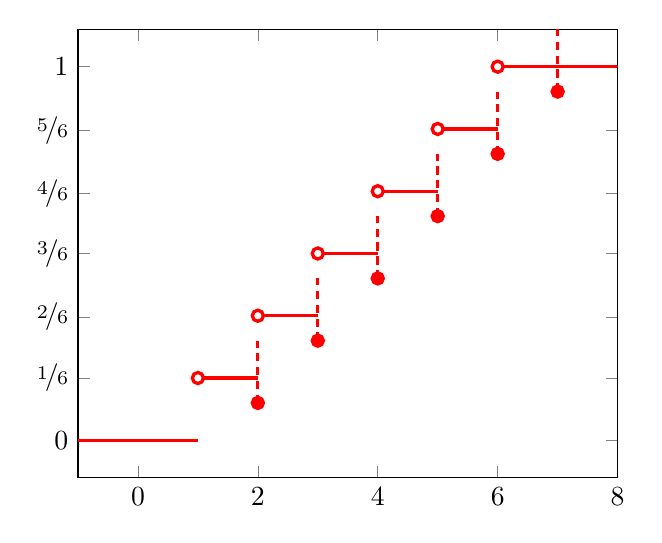
\begin{tikzpicture}
		\begin{axis}[
			jump mark left,
			ymin=-0.1, ymax=1.1,
			xmin=-1, xmax=8,
			ytick={0.0,0.166667,0.33,0.50,0.66,0.83,1.0},
			yticklabels={$0$, $\nicefrac{1}{6}$,$\nicefrac{2}{6}$,$\nicefrac{3}{6}$,$\nicefrac{4}{6}$,
					$\nicefrac{5}{6}$,$1$},
			every axis plot/.style={very thick},
			discontinuous,
			table/create on use/cumulative distribution/.style={
				create col/expr={\pgfmathaccuma + \thisrow{f(x)}}
			}
		]
		
			%TODO data is here - list the probabilities of each possible value of x
			\addplot [red] table [y=cumulative distribution]{
				x f(x)
				-1 0
				0 0
				1 1/6
				2 1/6
				3 1/6
				4 1/6
				5 1/6
				6 1/6
				7 0
				8 0
			};
		\end{axis}
	\end{tikzpicture}
\end{document}
